\documentclass{beamer}\usepackage[]{graphicx}\usepackage[]{color}
%% maxwidth is the original width if it is less than linewidth
%% otherwise use linewidth (to make sure the graphics do not exceed the margin)
\makeatletter
\def\maxwidth{ %
  \ifdim\Gin@nat@width>\linewidth
    \linewidth
  \else
    \Gin@nat@width
  \fi
}
\makeatother

\definecolor{fgcolor}{rgb}{0.345, 0.345, 0.345}
\newcommand{\hlnum}[1]{\textcolor[rgb]{0.686,0.059,0.569}{#1}}%
\newcommand{\hlstr}[1]{\textcolor[rgb]{0.192,0.494,0.8}{#1}}%
\newcommand{\hlcom}[1]{\textcolor[rgb]{0.678,0.584,0.686}{\textit{#1}}}%
\newcommand{\hlopt}[1]{\textcolor[rgb]{0,0,0}{#1}}%
\newcommand{\hlstd}[1]{\textcolor[rgb]{0.345,0.345,0.345}{#1}}%
\newcommand{\hlkwa}[1]{\textcolor[rgb]{0.161,0.373,0.58}{\textbf{#1}}}%
\newcommand{\hlkwb}[1]{\textcolor[rgb]{0.69,0.353,0.396}{#1}}%
\newcommand{\hlkwc}[1]{\textcolor[rgb]{0.333,0.667,0.333}{#1}}%
\newcommand{\hlkwd}[1]{\textcolor[rgb]{0.737,0.353,0.396}{\textbf{#1}}}%
\let\hlipl\hlkwb

\usepackage{framed}
\makeatletter
\newenvironment{kframe}{%
 \def\at@end@of@kframe{}%
 \ifinner\ifhmode%
  \def\at@end@of@kframe{\end{minipage}}%
  \begin{minipage}{\columnwidth}%
 \fi\fi%
 \def\FrameCommand##1{\hskip\@totalleftmargin \hskip-\fboxsep
 \colorbox{shadecolor}{##1}\hskip-\fboxsep
     % There is no \\@totalrightmargin, so:
     \hskip-\linewidth \hskip-\@totalleftmargin \hskip\columnwidth}%
 \MakeFramed {\advance\hsize-\width
   \@totalleftmargin\z@ \linewidth\hsize
   \@setminipage}}%
 {\par\unskip\endMakeFramed%
 \at@end@of@kframe}
\makeatother

\definecolor{shadecolor}{rgb}{.97, .97, .97}
\definecolor{messagecolor}{rgb}{0, 0, 0}
\definecolor{warningcolor}{rgb}{1, 0, 1}
\definecolor{errorcolor}{rgb}{1, 0, 0}
\newenvironment{knitrout}{}{} % an empty environment to be redefined in TeX

\usepackage{alltt}
\usepackage{listings}
%%to show python code in color
\usepackage[utf8]{inputenc}

%%usepackage{minted}  this didn't work to run python code
%%more to bring python code in color
\usepackage{color}
 
\definecolor{codegreen}{rgb}{0,0.6,0}
\definecolor{codegray}{rgb}{0.5,0.5,0.5}
\definecolor{codepurple}{rgb}{0.58,0,0.82}
\definecolor{backcolour}{rgb}{0.95,0.95,0.92}
 
\lstdefinestyle{mystyle}{
    backgroundcolor=\color{backcolour},   
    commentstyle=\color{codegreen},
    keywordstyle=\color{magenta},
    numberstyle=\tiny\color{codegray},
    stringstyle=\color{codepurple},
    basicstyle=\footnotesize,
    breakatwhitespace=false,         
    breaklines=true,                 
    captionpos=b,                    
    keepspaces=true,                 
    numbers=left,                    
    numbersep=5pt,                  
    showspaces=false,                
    showstringspaces=false,
    showtabs=false,                  
    tabsize=2
}
 
\lstset{style=mystyle}
%%end lines needed for color python code
\IfFileExists{upquote.sty}{\usepackage{upquote}}{}
\begin{document}

\title{The 9522: A python project}
\title{Data 520 Introduction to Programming \\
The 9522: A python project}
\author{Heidi Beezub}

\begin{frame}
  \titlepage
\begin{figure}
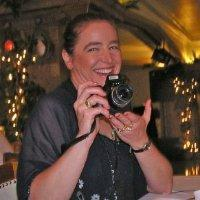
\includegraphics[scale=0.5]{profilePic}
\caption{Beezub}
\end{figure}
\end{frame}

\begin{frame}
  \frametitle{Outline}
    \tableofcontents
\end{frame}


\section{Background}
\begin{frame}[fragile]
  \frametitle{The 9522 and Rejects}
      \begin{itemize}
      \item<1->
        The DCM 9522 is one of the reports I use in order to correct 'rejects' in my job.  DCM stands for Department Cost Manager.  It includes multiple departments and all the products (both supplies and services) that each department provides.

      \item<2->
\textbf{What is a reject?}

   A reject is data that the system collects but then cannot process or put into the correct category.  Rejects are typically a 'new' item that simply needs the interface created or built in the system.  Sometimes this is an existing item that is coming into the system in a new way and needs an additinal interface.
    \item<3->
\textbf{What is an interface?}
The interface matches the data into the correct department. The system matches the product information (feeder key and feeder system).  

    \end{itemize}
  


\end{frame}

\begin{frame}[fragile]
  \frametitle{9522 could be better}
  \begin{itemize}  
\item<1->
    The 9522 helps me to determine if this is an existing item for which I need to create an additional interface. Or if it is a new product, which means I need to create the new product (including the interface).
\item<2->
    The report is \textbf{unwieldy} (6,600 pages).  I have to save the text file as a word file and then search the word file for the feeder key, IP number, or description information.  Since this is typically numerical it can result in multiple 'hits' many for the wrong field.  I also cannot easily compare the multiple hits in the word file. 
\item<3->
As an excel file I would be able to search on the columns and view any similar items (all at the same time).  It helps in identifying items to see what department(s) similar items are used in.  

\end{itemize}
  
\end{frame}

\section{Methodology}
\begin{frame}[fragile]
  \frametitle{Methodology}
\begin{itemize}  
\item<1->
\textbf{Source data}
My first step was to take a VERY critical look at the structure of the report.
The report includes headers on each page which can bisect the data at any point.  In addition to the information I want, the data also includes data I don't want that is part of the Bill of Materials.
\item<2-> 
\textbf{The desired end result}
A csv (excel file) that I will be able to filter to check items, sort to identify duplicate products and otherwise manipulate the data. With the goal being a better, more accurate and consistent database.
\item<3-> 
\textbf{Pseudocode}
First, I wrote down (pen & paper) what I needed to do.

\end{itemize}

\end{frame}

\section{Pseudocode}
\begin{frame}[fragile]
  \frametitle{Pseudocode}
  
\begin{figure}
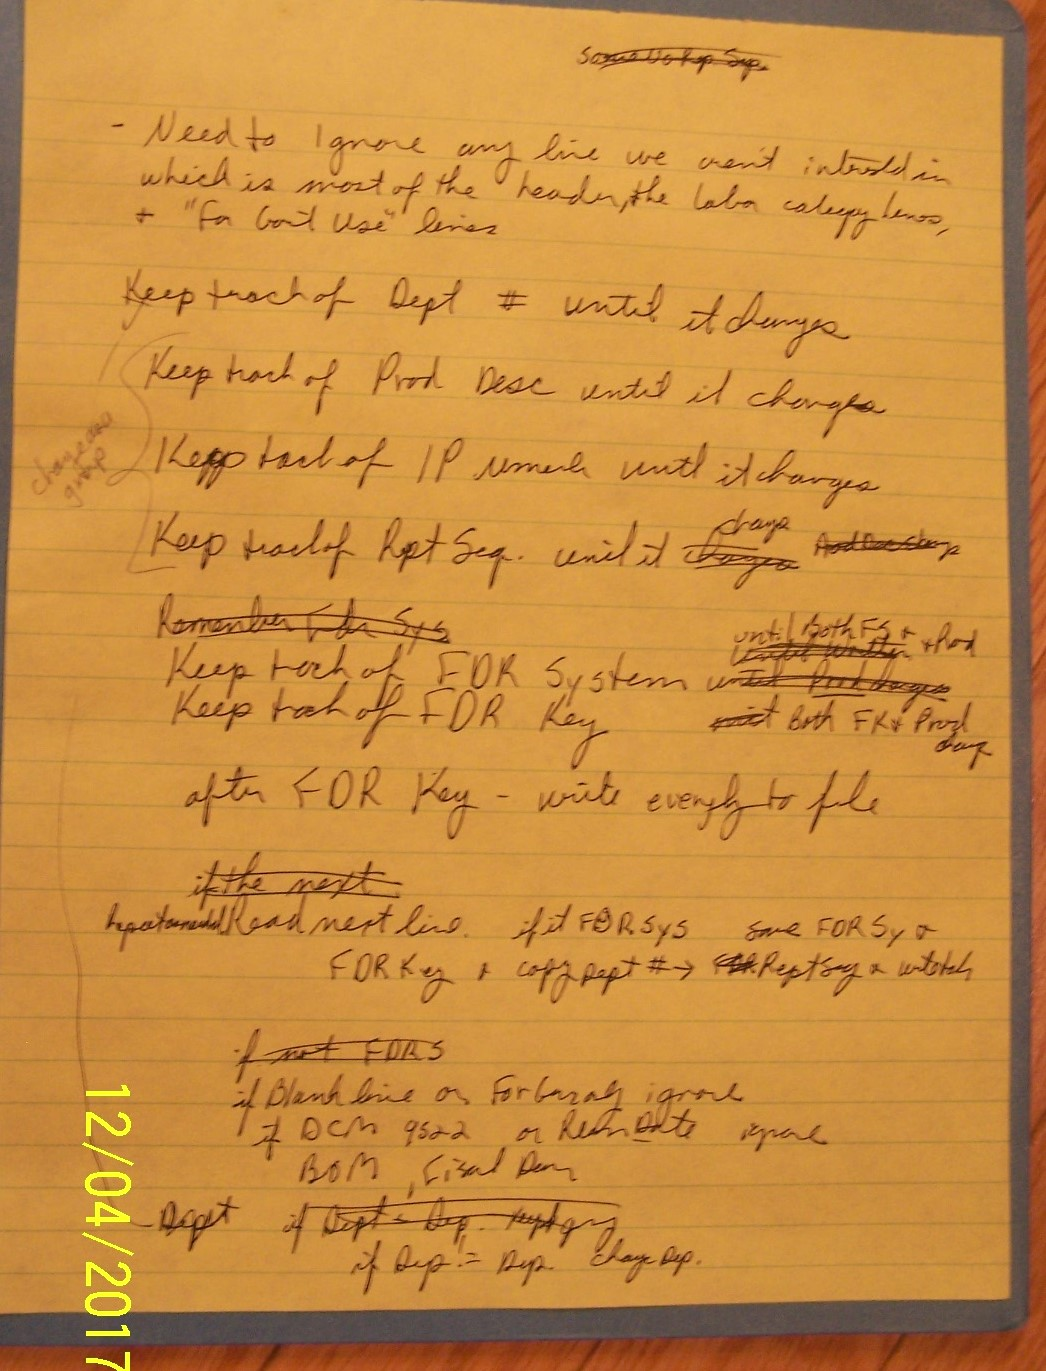
\includegraphics[scale=0.5]{pseudocode}
\caption{9522 pseudocode}
\end{figure}
  
\end{frame}

\section{9522}
\begin{frame}[fragile]
  \frametitle{9522 pre}
  
\begin{figure}
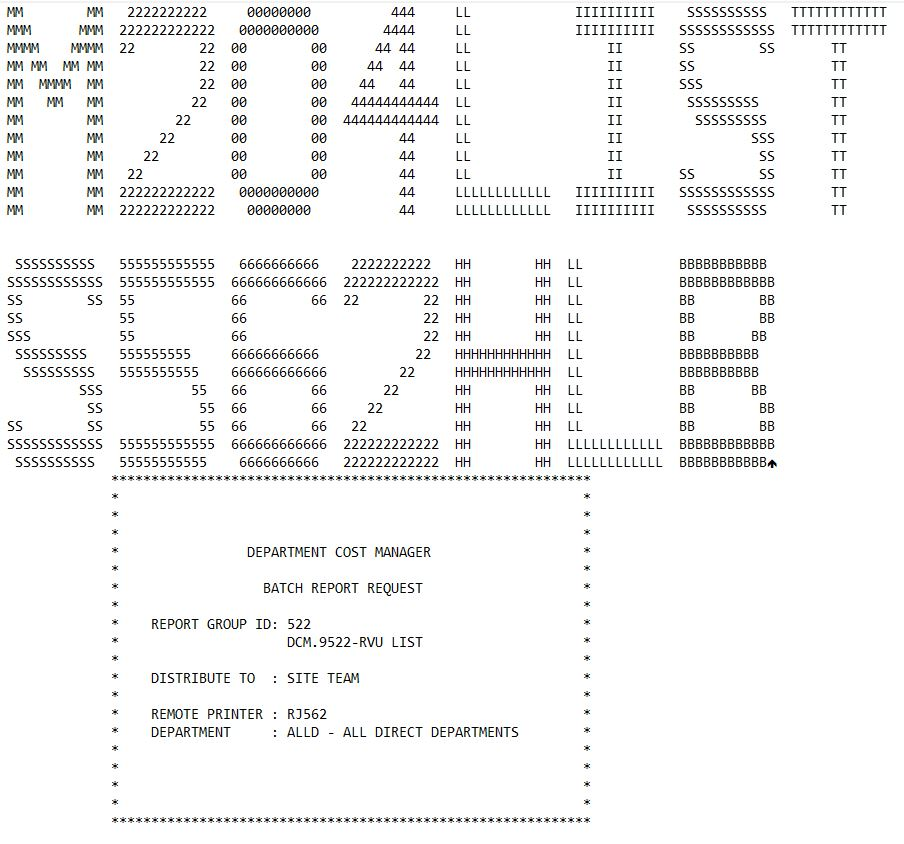
\includegraphics[scale=0.4]{9522_preamble}
\caption{9522 'preamble'}
\end{figure}
  
\end{frame}

\begin{frame}[fragile]
  \frametitle{9522 page 1}
  
\begin{figure}
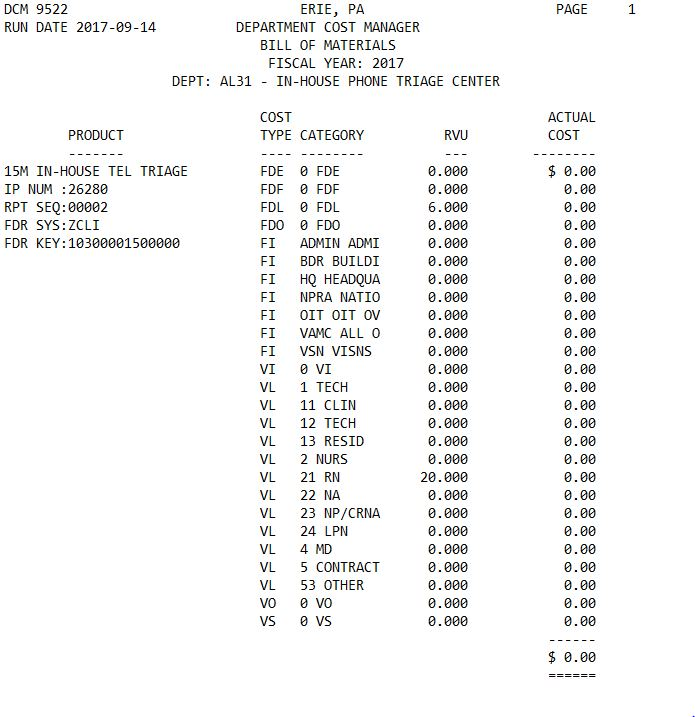
\includegraphics[scale=0.4]{9522_page1}
\caption{9522 page 1}
\end{figure}
  
\end{frame}


\begin{frame}[fragile]
  \frametitle{9522 header bisects data}
  
\begin{figure}
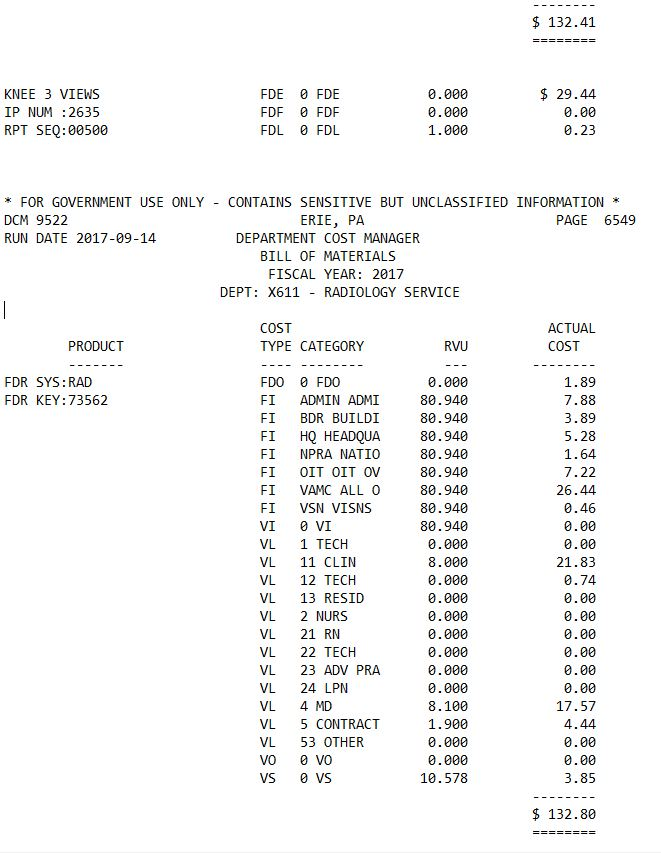
\includegraphics[scale=0.4]{9522_bisect}
\caption{9522 page 1}
\end{figure}
  
\end{frame}


\begin{frame}[fragile]
  \frametitle{9522 page 6636}
  
\begin{figure}
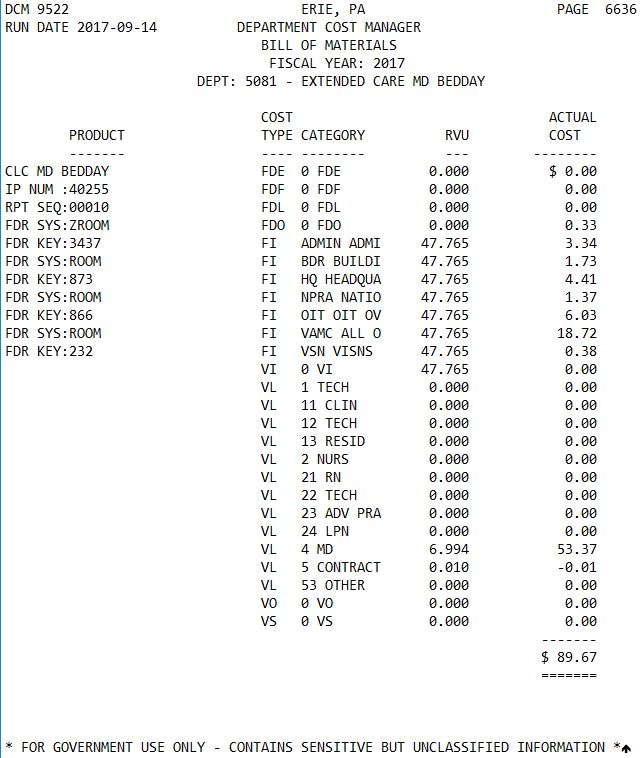
\includegraphics[scale=0.4]{9522_page6636}
\caption{9522 page 1}
\end{figure}
  
\end{frame}


\section{Code for IP Number}
\begin{frame}[fragile]
  \frametitle{Code for IP Number}
I wanted to start small and to start in the 'middle' of my code. Each line of text is read into a list and I use the position in the list to extract the data.
  %%\lstinputlisting[language=Python]{9522_slide_IPNUM_only.py} inputs code direct from file
  %%\inputminted{python}{9522_slide_IPNUM_only.py}
%%framebreak won't work with the lstlisting for language =python   
\begin{lstlisting}[language=Python]

def process_file(reader):
    result_line= ''
    result=''
    #first we need to add headers
    
    with open('9522_new.csv', 'a') as output_file:
        output_file.write('"DEPT","PRODUCT","IPNUM","RPTSEQ","FDRSYS","FDRKEY"' +'\n')
    for line in reader:
        line=line.strip()    #removes leading/trailing whitespace
        field = line.split()
\end{lstlisting}
        
%%echo python_name-no.py    cntl+enter
%%control+shift+enter   needs to be a .py file in Rstudio

   
\end{frame}

\begin{frame}[fragile]
  \frametitle{Code for IP Number continued}
  %%\lstinputlisting[language=Python]{9522_slide_IPNUM_only.py} inputs code direct from file
  %%\inputminted{python}{9522_slide_IPNUM_only.py}
%%framebreak won't work with the lstlisting for language =python  
Here is the code I used to extract the IP Number:

\begin{lstlisting}[language=Python]
if len(field)>3:
      for i in range(0,2):
         #find IPNUM
        if field[i] == 'IP' and field[i+1] =='NUM':
             #save IPNUM
            ipnum=field[i+2].strip(':')

\end{lstlisting}
%indents off to save slide space
%%echo python_name-no.py    cntl+enter
%%control+shift+enter   needs to be a .py file in Rstudio
  
   
\end{frame}

\section{Code for Sequence Number and Feeder System}
\begin{frame}[fragile]
  \frametitle{Code for Sequence Number and Feeder System}
I added code one item at a time, this not only made sure I didn't break what I already had, but also allowed me to debug after each step in the process.

\textbf{Selected code to pull each item:}

\begin{lstlisting}[language=Python]
    #find RPT Seq
    if field[i] == 'RPT' and field[i+1].startswith('SEQ:'):
        #save RPT SEQ
        rptseq =field[i+1].strip('SEQ:')
    #find FDR SYS
    if field[i] == 'FDR' and field[i+1].startswith('SYS:'):
        #(Kudgel) strip SYS deletes the leading/trailing S from the fdrsys
        if field[i+1] == 'SYS:SUR':
            #save FDR SYS
            fdrsys='SUR'
        else:
            #save FDR SYS
            fdrsys=field[i+1].lstrip('SYS:')  #lstrip accounts for ECS fdr system
\end{lstlisting}
   
\end{frame}

\section{Code for Feeder Key}
\begin{frame}[fragile]
  \frametitle{Code for Feeder Key}
The \textbf{feeder key} is the 'last' item before the line can be written to the file.  The majority of Feeder Keys are one 'word'/text string without breaks, however there were a handful of cases where the Feeder Key was more than one text string.

\begin{lstlisting}[language=Python]
    #find FDR KEY (last item before write to file)
if field[i] == 'FDR' and field[i+1].startswith('KEY:'):
        #(Kudgel)save FDR KEY
        if field[i+2] == 'COST':   #for 'MEDIUM COST' fdrkey
            fdrkey=field[i+1].lstrip('KEY:') + ' COST'
        elif field[i+2] == 'DRUG':
            fdrkey=field[i+1].lstrip('KEY:') + ' DRUG '+ field[i+3]
        else:
            fdrkey=field[i+1].lstrip('KEY:') #lstrip accounts for 'E'in fdrkey
      
\end{lstlisting}
   
\end{frame}


\section{Product Description}
\begin{frame}[fragile]
  \frametitle{Product description}
The \textbf{product description} was more challenging.  There were no key words at the beginning of the line.  I would have to keep track of a prior line to know when the next line would be the product description.  This is where familiarity with the data was key.  At the very END of each Bill of Materials was an "=" line.  However, this doesn't help for the very first item.

I used 'counters' to keep track of when I came to the end of one item (the '=' line).  And also to process the very first item.


\end{frame}

\section{Product Description Code-first item}
\begin{frame}[fragile]
  \frametitle{Product description Code-first item}

\begin{lstlisting}[language=Python]
                if field[i] == first_var:
                    first_count = 1
                    prod=''
                    break          
                #find first prod desc
                if first_count == 1:
                    #after first item update first_var
                    first_var='datasci'
                    for f in range(len(field)):
                        if field[f]=='FDE':
                      #don't want any info after FDE
                            first_count=10
                            break
                        else:
                            prod=prod+field[f]+' '
                            #redundant
                            count=0
                            first_count=10
\end{lstlisting}


\end{frame}

\begin{frame}[fragile]
  \frametitle{9522 page 1}
  
\begin{figure}
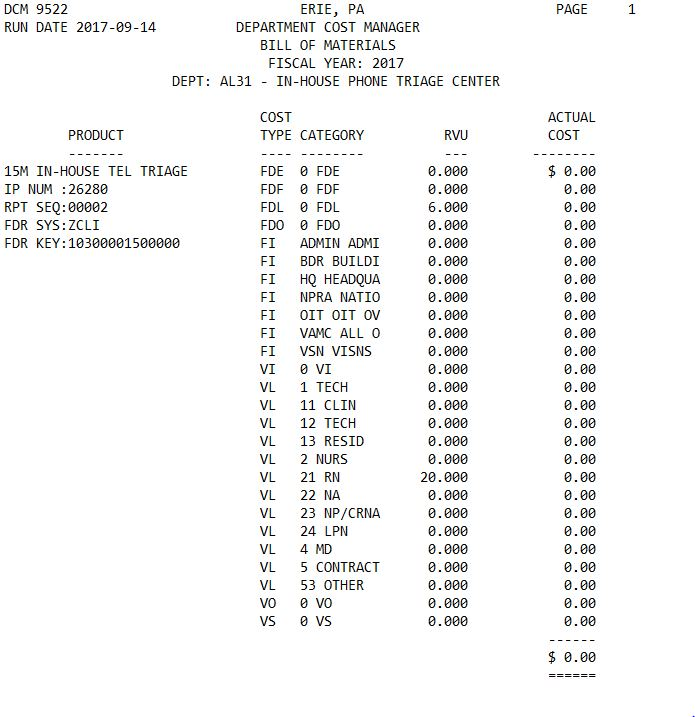
\includegraphics[scale=0.4]{9522_page1}
\caption{9522 page 1}
\end{figure}
  
\end{frame}


\section{Product Description Code-other items}
\begin{frame}[fragile]
  \frametitle{Product description Code-other items}

\begin{lstlisting}[language=Python]
          #find prod desc
      #'hardcode' in the startswith field[0] instead of using i
      if (count >0 and not field[0].startswith('*') and not field[0].startswith('DCM')
              and not field[0].startswith('RUN')and not field[0].startswith('BILL') and not
              field[0].startswith('FISCAL') and not field[0].startswith('DEPT:') and not
              field[0].startswith('PRODUCT')and not field[0].startswith('-------')):
          ##print ('count at not *=',count)
          ##print('field[i]=',field[i])
          ##print('field=',field)
          for d in range(len(field)):
              if field[d]=='FDE':
                  #don't want any info after FDE
                  count=0
                  break
              else:
                  prod=prod+field[d].replace(","," ")+' '
                  #https://www.safaribooksonline.com/library/view/python-cookbook-3rd/9781449357337/ch02s11.html
                  #the replace() method or a regular expression substitution.
                      #redundant
                      count=0

\end{lstlisting}

\end{frame}

\begin{frame}[fragile]
  \frametitle{9522 header bisects data}
  
\begin{figure}
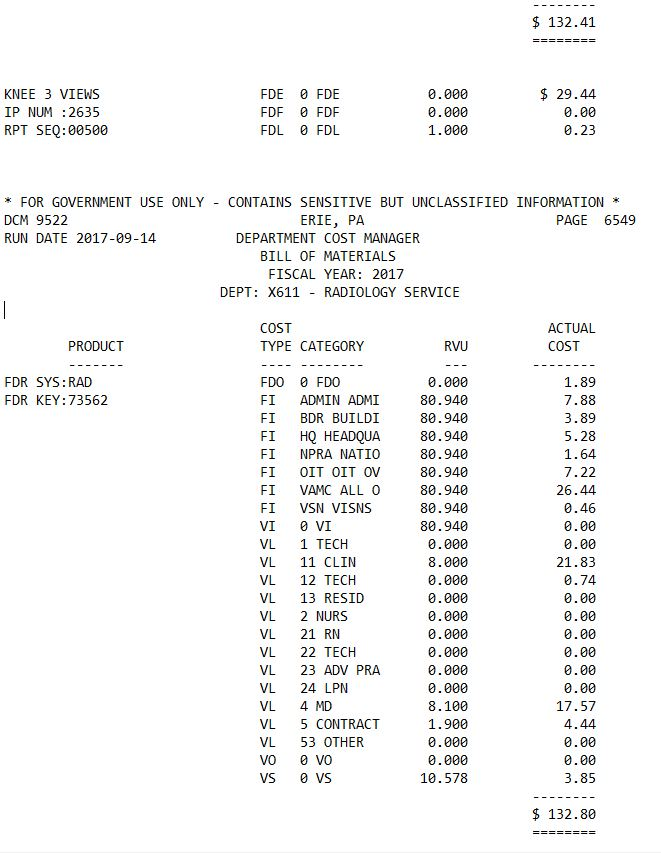
\includegraphics[scale=0.4]{9522_bisect}
\caption{9522 page 1}
\end{figure}
  
\end{frame}

\section{Debugging}
\begin{frame}[fragile]
  \frametitle{Debugging}
\begin{itemize}  
\item<1->
\textbf{Starting small} with 6,000 pages and 14,500 products (as it turns out) using the entire report to develop the code would have taken a substantial amount of time.  So in the same way that I added code one item at a time, I started with a small truncated report and then used larger and larger portions of the report until I finally was using the entire report.
\item<2->
My debugging during the main writing phase was based on the minimal \textbf{37 page} report.
Once I had my code complete (or so I thought) I expanded my source data to 127 pages (looking for 'natural' product information ends at the end of a page).  Again more debugging.
\item<3->
The next expansion was 500 pages followed by ('surprise') more debugging.  The next tests were at 1,000 then 2,000 and 3,000 pages followed by (you guessed it) more debugging.

\end{itemize}


\end{frame}

\begin{frame}[fragile]
\frametitle{Additional Debugging}
\begin{itemize}  
\item<1->
After the initial code was written, debugging mainly consisted of finding 'special' cases that did not conform to the 'normal' data.  Most of these were relatively easily fixed by adding code that looked for these special cases.   During testing I reviewed the csv file data to insure the formatting and data was accurate.  This involved not only 'eyeballing' the data but also section comparison between the 9522 and csv file to insure accuracy.
\item<2->
I then jumped to the full 6,600 page report data I was surprised to find I still had debugging to perform.  
\item<3->

\textbf{Final testing} To verify that I was capturing all of the items and multiple feeder system/key pairs.  I choose four 50-page blocks of the report (first 50, last 50 and two 50's in the middle). I verified textbf{line by line} that everything was in the csv file as it should be.  This step also identified additional 'special' conditions.  After accounting for these items, I again did a line by line verification for the first & last 50 pages, the 50-page segment that 'failed' and then a new 50-page section.

\end{itemize}
\end{frame}

\section{Mis-steps and wrong directions}
\begin{frame}[fragile]
\frametitle{Mis-steps and wrong directions}
\begin{itemize}  
\item<1->
Really focus on \textbf{small}: When I first started coding, even though I had in my mind to only do a little, I still did too much.  I cut back and had to focus on the one item (and then adding one item at a time).
\item<2->
I started off using functions to read and write to the file and to extract the items, however, when I got to the product description I had to totally change: I needed to be able to save and 'remember' a variable which I can't do between functions.  So I needed to switch to one continuous function.
\item<3> 
\textbf{My own genius}: I am proud of myself for the way I handle finding the first line after the header (without getting any other line after the header).  By defining the '---' (dash line) through a variable, I could then change the variable so it would never find the dash line again.

\end{itemize}

\end{frame}


\begin{frame}[fragile]
\frametitle{Final notes}
\begin{itemize}  
\item<1->
Verification debugging was the \textbf{worst}.  But I knew I needed to power through it one line of data and one line of source code at a time. 
\item<2->
I should have kept a notebook to keep track of everything I did.  Specifically I wish I knew which pages I used for line by line checks. 
\item<3> 
My next step will be to start using this for my rejects and get the 9522 from other stations (other VAs) to see how it works with other reports (data nomenclature is not standardized).  I may need to re-write my code to focus on the FI, VL, FDL, etc. lines depending on how other hospitals enter their data.

\end{itemize}

\end{frame}

\end{document}
